\chapter{Équations différentielles à condition initiale}

\section{Problème de Cauchy}

$f : [a,b] \times \R^n \longrightarrow \R^n$ de classe $\mathcal{C}^0$

\begin{equation*}
    \begin{array}{cc}
        \boxed{\begin{aligned}
            y'(t)  & = & f(t,y(t)) \\
            y(t_0) & = & y_0 \\
            t \in [a,b]
        \end{aligned}}
        & \hspace{1cm}
        \parbox{5cm}{\textbf{Problème différentiel de condition initiale (problème de Cauchy})}
    \end{array}
\end{equation*}

où $[a,b] \subset \R$

\hspace{0.5cm} $y : t \in [a,b] \longrightarrow y(t) \in \R^n$ application dérivable inconnue

\hspace{0.5cm} $f : (t, \theta) \in [a,b] \times \R^n \longrightarrow f(t,\theta)$ aplpication donnée

\hspace{0.5cm} $y_0$ : valeur initiale donnée


Résoudre le problème c'est donc déterminer une application $y$, si elle existe, qui est solution de 
l'équation différentielle $y'(t) = f(t,y(t))$ et qui prend la valeur numérique donnée 
$y_0$ à l'instant initial $t=t_0$

\subsection*{Domaines d'application :}
\begin{enumerate}[label=-]
    \item mécanique
    \item système solaire ($\to$ modélisation par des lois de Newton, $n \geq 3$ pas de solution analyitique)
    \item cinétique chimique ($\to$ réaction chaotiques)
    \item météo ($\to$ évolution des champs de pression à la surface de la Terre, turbulences)
    \item Animation d'objets 3D par ordinateur
\end{enumerate}

\subsection*{Résolutions numériques des EDO}
\begin{enumerate}[label=*]
    \item Les erreurs de troncature ne sont pas négligeables quand on a beaucoup d'itérations
    \item Convergence
        \begin{figure}[h]
            \centering
            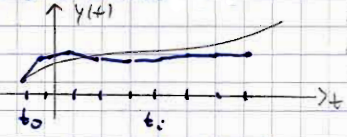
\includegraphics[scale=0.5]{5-EDO-cvgence.png}
            \caption{Calcul de $n$ valeurs approchées}
        \end{figure}
    \item Stabilité : petites perturbations à l'entrée restent bornées à la sortie ?
    \item Consistance : erreur locale doit tendre vers 0 pour $h \to 0$.
    \item Chaos : une faible perturbation sur les CI peut entraîner une divergence de la solution.
\end{enumerate}

\begin{ftheo}[Cauchy-Lipschitz : Existence + Unicité]
    Soit $f : [a,b] \times \R^n \longrightarrow \R^n$ de classe $\mathcal{C}^0$ et vérifiant
    la propriété suivante :

    Il existe une constante $L \in \R$ telle que :
        \begin{equation*}
            \forall t \in [a,b], \forall y_1, y_2 \in \R^n, \hspace{1cm} \norm{f(t,y_1) - f(t,y_2)} \leq L \norm{y_1 - y_2}
        \end{equation*}

        Alors quelque soit $t_0 \in [a,b]$ et $y_0 \in \R^n$, il existe une unique fonction
        $y : [a,b] \longrightarrow \R^n$ avec
    \begin{enumerate}[label=(\roman*)]
        \item $y(t)$ est de classe $\mathcal{C}^1$ sur $[a,b]$
        \item $y'(t) = f(t,y(t))$ pour $t \in [a,b]$
        \item $y(t_0) = y_0$
    \end{enumerate}
\end{ftheo}

Dans la suite on se restreint au cas d'\textbf{une} équation ($n=1$) différentielle.
\vspace{0.5cm}

\begin{exemple}[Méthode d'Euler]
    On subdivise $[a,b]$ en $n$ intervalles de longueur \\ $h = \displaystyle\frac{b-a}{N}$, $t_i = a+ih$, $i=0,\dots,N$

    La méthode d'Euler consiste à calculer par récurrence des valeurs approchées
    $y_1, \dots, y_N$ de $y(t_1), \dots, y(t_N)$ respectivement au moyen de la formule suivante :
    \[
        y_{k+1} = y_k + h f(t_k,y_k) \hspace{1cm} k=0,\dots,N-1
    \]

    L'idée de la méthode est alors de considérer que sur le petit intervalle $[t_0,t_{0+h}]$ la
    courbe n'est pas très éloignée de sa tangente en $t_0$

    \[
        \begin{split}
            \frac{y(t_0 + h) - y(t_0)}{h} \approx \; & f(t_0,y(t_0)) \\
            y(t_0 + h) \approx \; & y(t_0) + h f (t_0, y(t_0)) \\
            y_1 = \; & y_0 + h f(t_0,y_0)
        \end{split}
    \]

    \vspace{1cm}

    \begin{figure}[h]
        \centering
        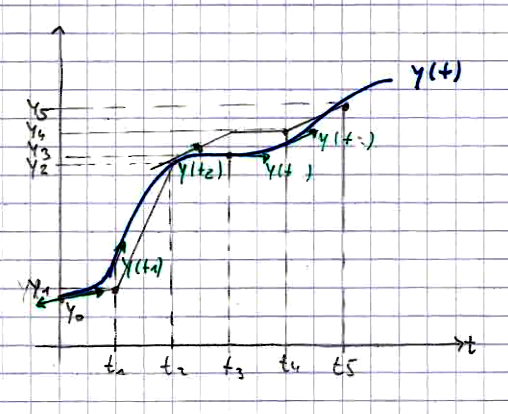
\includegraphics[scale=0.42]{5-EDO-euler.png}
    \end{figure}

    Partant de $t_0 = a$, on connaît $y_0 = y(t_0)$ donc aussi la dérivée en ce point $f(t_0,y_0)$

\end{exemple}

\textbf{Convergence :}

On fixe un \textbf{point $\tilde{t}$} et on regarde le comportement de l'erreur $e_k = y_k - y(t_k)$
en diminuant $h_j = \displaystyle\frac{b-a}{j}$ ($h \to 0$ pour $j \to + \infty$). On voudrait que
les valeurs approximatives $y_k$ tendent vers $y(t_k)$ si $h$ tend vers 0 :
$| y_k - y(t_k) | \leq C.h$

\begin{ftheo}[Convergence d'Euler]
    On suppose vérifiées les hypothèses ``Cauchy-Lipschitz'' et que la solution $y$ du problème 
    de Cauchy appartient à $\mathcal{C}^2[a,b]$

    On pose $M_2 = \underset{t\in[a,b]}{\Max} |y''(t)|$

    Alors si on note $e_k = y_k - y(t_k)$ l'erreur au point $t_k$, on a la majoration
    \[
        |e_k| \leq \underbrace{\frac{1}{L} (e^{L(b-a)}-1) \frac{M_2}{2}h}_{\text{$= c$ ne dépend pas de $t_k$}}
    \]
    \[
        |e_k| \leq C.h
    \]
\end{ftheo}

\begin{preuve}
    Comme $y \in \mathcal{C}^2[a,b]$ on a en particulier la formule de Taylor :
    \begin{equation}
        \begin{aligned}
            & y(t_k + h) = y_k(t_k) + h y'(t_k) + \frac{1}{2}h^2 y''(\xi) \\
            \iff & y(t_{k+1}) = y(t_k) + h +f(t_k, y(t_k)) + \frac{1}{2}h^2 y''(\xi)
        \end{aligned}
            \tag{*}
    \end{equation}

    Soustrayons donc :
    \begin{align*}
        y_{k+1} = & y_k + hf(t_k,y_k) \\
        - (*) & 
    \end{align*}

    On obtient :
    \[
        e_{k+1} = e_k + h \Big[ f(t_k,y_k) - f(t_k, y(t_k)) \Big] - \frac{1}{2}h^2 y''(\xi)
    \]

    En appliquant ``Cauchy-Lipschitz'' :
    \begin{equation}
        |e_{k+1}| \leq |e_k| (1 + Lh) + \frac{1}{2}h^2 M_2 \hspace{1cm} 0 \leq k \leq N-1
        \tag{**}
    \end{equation}
\end{preuve}

\begin{lemme}
    Soit $(\varepsilon_k), k=0,\dots,N$ une suite de nombres positifs vérifiant :
    \[
        \varepsilon_{k+1} \leq \varepsilon_k a + b \hspace{1.5cm} k=0,\dots,N-1
    \]

    Alors :
    \[
        \varepsilon_k \leq \varepsilon_0 \; a^k + b \frac{a^k - 1}{a - 1}
    \]
\end{lemme}
\begin{preuve}
    Immédiate par récurrence.
\end{preuve}

\begin{lemme}
    Pour tout $k \in \N$ et tout réel $u \geq u$ on a :
    \[
        (1+u)^k \leq e^{ku}
    \]
    \label{eqdiff:lemme1}
\end{lemme}

\begin{preuve}
    Il suffit de montrer que $1+u \leq e^u$.

    Posons $z(u) = 1 + u - e^u$, on a $z'(u) = 1 - e^u$

    $z'$ est négatif et donc $z$ est décroissant sur $[0,+\infty[$

    Or $z(0) = 0 \implies 1 + u - e^u \leq 0 \implies$ d'où le résultat.
    \label{eqdiff:lemme2}
\end{preuve}

Lemme \ref{eqdiff:lemme1} appliqué à (**) donne (puisque $e_0 = 0$, CI) :
\[
    \abs{e_k} \leq 0.(1+Lh)^k + \frac{h^2M}{2}\frac{(1+Lh)^k - 1}{Lh} = \frac{4M2}{2L}
\]

On applique alors \ref{eqdiff:lemme2} :
\[
    \abs{c_k} \leq \frac{e^{Lhk}-1}{L}.\frac{M_2}{2}h
\]

et $kh=t_k-a \leq b-a$ donc :
\[
    \abs{e_k} \leq \frac{e^{L(b-a)}-1}{L}.\frac{M_2}{2}h
\]

\hspace{1cm}

On a donc la convergence, mais qu'en est-il de la stabilité et de la consistance ?

\hspace{1cm}

\subsection*{2 classes de méthodes :}
\begin{enumerate}[label=(\arabic*)]
    \item À pas séparé \textbf{MPS} : $y_{k+1}$ approximation de $y(t_{k+1})$ est calculé à partir de $y_k$
    \item À pas multiple \textbf{MPM} : $y_{k+1}$ est calculé à partir de plusieurs
        points précédents $y_k,y_{k-1},\dots,y_{k-p}$.
\end{enumerate}

\section{Méthodes à pas séparé}
``Schéma à un pas''

\subsection{Définition}

\vspace{-0.5cm}

\begin{equation*}
    \left\lbrace
    \begin{array}{c}
        y'(t) = f(t,y(t)) \\
        y(a) \; \text{ donné}
    \end{array}\right.
\end{equation*}

$f$ continue, lipschitzienne par rapport à $y$ $\implies$ $\overline{y}$ solution uique au problème de Cauchy.

\subsection*{But :}
Approcher $\overline{y}(t_k)$ aux points $t_k = a + kh$

$h=\displaystyle\frac{b-a}{N}$ pas constant, $t_0=a, t_n=b$, $k=0,\dots,N$

\begin{fdef}[MPS]
    Une \textbf{MPS} est un schéma itératif de la forme :
    \[
        y_{k+1} = y_k + h \; \Phi(t_k,y_k,h)
    \]

    $y_0$ donné : $y_0 = \overline{y}(a)$

    $t_{k+1} = t_k + h$
\end{fdef}

\begin{exemple}
    Euler $\Phi(t,y,h) = f(t,y)$

    Ici $\Phi$ est indépendant de $k$.

    On dira que $\Phi$ définit la MPS.
    On appelle \textbf{erreur} au point $t_k$ : $e_k = y_k - \overline{y}(t_k)$

    \textbf{Le but} est de construire des MPS (i.e. $\Phi$) telles que 
    \[
        \Max \abs{e_k} \xrightarrow{h\to0} 0
    \]
    \begin{center}
        i.e.
    \end{center}
    \[
        \Max \abs{e_k} = \gO (h^p) \hspace{1cm} p\in\N
    \]

    Plus $p$ est grand, plus la méthode converge vite.
\end{exemple}

\subsection{Consistance, stabilité et convergence}

\begin{fdef}
    On dit que la \textbf{MPS} est \textbf{convergente} si :
\[
    \forall y_0 \in \R, \lim_{\underbrace{h\to0}_{\text{erreur en un pt $t_k \to 0$}}} \Max_{k\in\{1,..,N\}} \abs{y_k - \overline{y}(t_k)} = 0
\]
\label{eqdiff:def1}
\end{fdef}

\begin{remark}
    On peut même aller plus loin dans la définition de la convergence en
    ne supposant pas que le schéma part de la condition initiale exacte.

    Autrement dit, la méthode doit converger même s'il y a une erreur
    (de troncature \dots) sur la condition initiale.

    Ce qui donne la :
\end{remark}

\begin{fdef}
    La MPS est \textbf{convergente} si :
    \[
        \lim_{y_0\to\overline{y}(a), h\to0} \Max_k \abs{y_k - \overline{y}(t_k)} = 0
    \]
    \label{eqdiff:def2}
\end{fdef}

On verra maintenant que la convergence résulte de deux propriétés :
\textbf{stabilité} et \textbf{consistance}.

\begin{enumerate}[label=$\to$]
    \item La \textbf{stabilité} est une propriété propre au schéma.
        Elle assure que le schéma n'amplifie pas trop les
        erreurs (numériques) que l'on commet à chaque pas.

        Schéma exactement calculé : $y_{k+1} = y_k + h \; \Phi (t_k,y_k,h)$ 
        
        $\ne$ schéma calculé par ordinateur :
        \begin{equation*}
            \left\lbrace
            \begin{array}{c}
                z_0 = y_0 + \varepsilon_0 \\
                z_{k+1} = z_k + h \big[ \Phi(t_k,z_k,h) + \varepsilon_k \big]
            \end{array}\right.
        \end{equation*}

        \begin{fdef}
            La méthode \textbf{MPS} est \underline{stable} si :
                $\exists M > 0, \exists \overline{\varepsilon} > 0$ t.q.

                \[
                    \forall h, \forall \varepsilon_i < \overline{\varepsilon} : \underset{k}{\Max} \abs{y_k-z_k} < M . \underset{i \in \{0,..,M-1\}}{\Max} \abs{\varepsilon_i}
                \]
        \end{fdef}

    \item La \textbf{consistance} définit une relation entre le schéma et l'équation
        différentielle. Elle implique que le schéma s'écarte peu localement de la
        solution.

        \begin{fdef}
            Une \textbf{MPS} est dite \textbf{consistance} avec l'équation différentielle si
            \[
                \abs{\underbrace{\frac{\overline{y}(t+h) - \overline{y}(t)}{h}}_{\Delta(t,\overline{y}(t),h)}
                - \Phi(t,\overline{y}(t),h)}
                \overset{h\to0}{\underset{N\to+\infty}{\longrightarrow}} 0
            \]
            \label{eqdiff:def3}
        \end{fdef}

        Autrement dit, si l'on veut que le schéma marche, il faut au minimum qu'il soit
        à peu près vérifié par la solution formelle $\overline{y}$ quand $h$ est assez
        petit $\iff \overline{y}(t+h) - \overline{y}(t) - h \; \Phi (t,\overline{y}(t),h) = \gO(h) \leq L.h$
\end{enumerate}

\begin{ftheo}[Th. Fondamental]
    \[
        \text{Stabilité + Consistance $\implies$ Convergence.}
    \]
\end{ftheo}

\begin{preuve}
    \[
        y_{k+1} = y_k + h \; \Phi(t_k,y_k,h)
    \]

    Idée : considérer la solution exacte $\overline{y}$ comme une perturbation de
    la solution numérique !

    \vspace{-0.5cm}
    \begin{align*}
        \overline{y}(t_{k+1}) & = \overline{y}(t_k) + h \; \Delta (t_k,\overline{y}(t_k),h) \\
        & = \overline{y}(t_k) + h \; \Phi (t_k, \overline{y}(t_k),h) + \varepsilon_k
    \end{align*}

    On pose $\varepsilon_k = [\Delta - \Phi]_k$

    \vspace{-0.5cm}
    \begin{align*}
        z_k & = \overline{y}(t_k) & y_0 & = z_0 \\
        z_{k+1} & = \overline{y}(t_{k+1})
    \end{align*}
    \[
        \implies \varepsilon_k = \frac{\overline{y}(t_{k+1}-\overline{y}(t_k)}{h} -
        \Phi(t_k,\overline{y}(t_k),h)
    \]

    Hypothèse de consistance $\implies \abs{\varepsilon_k} \overset{h\to0}{\longrightarrow} 0$

    Hypothèse de stabilité $\implies \exists M, \exists \overline{\varepsilon} > 0 \text{ t.q }
    \forall \varepsilon_i < \overline{\varepsilon} :$
    \[
        \Max \abs{y_k - \overline{y}(t_k)} < M.\underset{k}{\Max} \abs{\varepsilon_k} \overset{h\to0}{\longrightarrow} 0
    \]

    Donc $\Max \abs{y_k - \overline{y}(t_k)} \overset{h\to0}{\longrightarrow} 0$

    Donc \textbf{MPS est convergente}.
\end{preuve}

\begin{remark}
    Réduire la démonstration de la convergence à la vérification de la consistance et
    de la stabilité a un double avantage :
    \begin{enumerate}[label=$-$]
        \item Un schéma stable qui n'est pas consistant calcule bien quelque chose, mais
            pas ce que l'on cherche.
        \item Un schéma instable mais consistant calcule une solution qui peut être proche
            initialemet de ce que l'on cherche, mais qui s'éloigne rapidement
            (souvent de façon oscillante).
    \end{enumerate}
\end{remark}

\subsection{Caractérisation de la consistance et de la stabilité}

On suppose que $\Phi$ est continue en $t\in[a,b], y \in \R$, et $h$, en $h=0$.

\begin{prop}
    MPS est consistante $\iff \Phi(t,y,0) = f(t,y)$.
\end{prop}

\begin{preuve}
    ``$\implies$'' MPS consistante 
    \begin{equation}
        \implies \abs{\underbrace{\frac{\overline{y}(t+h) - \overline{y}(t)}{h}}_{\overline{y}'(t) + o(t)}
        - \Phi(t,\overline{y}(t),h)} \overset{h\to0}{\longrightarrow} 0
        \tag{*}
    \end{equation}

    Soit $\varepsilon > 0$ :
        \begin{align}
            \overline{y} \in \mathcal{C}^1 & \implies \exists h_0 : \forall h < h_0
            \abs{\frac{\overline{y}(t+h)-\overline{y}(t)}{h} - \overline{y}'(t)} < \frac{\varepsilon}{2}
            \notag
            \\
            & \implies \frac{\overline{y}(t+h) - \overline{y}(t)}{h} - \frac{\varepsilon}{2} < f(t,y(t)) < \frac{\overline{y}(t+h) - \overline{y}}{h} + \frac{\varepsilon}{2}
            \tag{*2}
        \end{align}

        \begin{align}
            (*) & \implies \exists h_1 : \forall h < h_1 \abs{\frac{\overline{y}(t+h) - \overline{y}(t)}{h} - \Phi(t,\overline{y}(t),h)} < \frac{\varepsilon}{2}
            \notag
            \\
            & \implies \frac{\overline{y}(t+h) - \overline{y}(t)}{h} - \frac{\varepsilon}{2} < \Phi(t,\overline{y}(t),h) < \frac{\overline{y}(t+h) - \overline{y}(t)}{h} + \frac{\varepsilon}{2}
            \tag{*3}
        \end{align}

        \vspace{0.5cm}
        $h_2 := \Min(h_0,h_1), \; \forall h < h_2$

        $(*2) - (*3) \implies \abs{f(t,\overline{y}(t) - \Phi(t,\overline{y}(t),h} < \varepsilon$

        \begin{equation}
            \implies \text{Pour $h \to 0$ : $f(t,y(t)) = \Phi(t,\overline{y}(t),0)$, car $\Phi$ continue.}
            \tag{*4}
        \end{equation}

        Maintenant, il faut montrer que l'égalité est vraie $\forall y$. (*4) est vraie pour
        tout y qui sont solution du problème de Cauchy. On peut donc appliquer (*4) à
        l'unique solution du problème de Cauchy 
        \[
            \left\lbrace
            \begin{array}{c}
                y(t_0) = y_0 \\
                y'(t) = f(t,y(t))
            \end{array}\right.
        \]
        $\implies$ On trouve $f(t_0,y_0,0) = f(t_0,y_0), \; \forall t_0,y_0$

        \vspace{1.3cm}
        ``$\Longleftarrow$'' :
        $\Phi(t,y,0) = f(t,y)$

        Comme $\Phi$ est continue en $h$ :
        \begin{equation}
            \Phi(t,y,h) \overset{h\to0}{\longrightarrow} \Phi(t,y,0) = f(t,y)
            \label{eqdiff:eqdemo1}
        \end{equation}

        Comme $\overline{y} \in \mathcal{C}^1$ :
        \begin{equation}
            \frac{\overline{y}(t+h) - \overline{y}(t)}{h} \overset{h\to0}{\longrightarrow}
            \overline{y}'(t) = f(t,y)
            \label{eqdiff:eqdemo2} 
        \end{equation}

        \[
            (\ref{eqdiff:eqdemo1}) - (\ref{eqdiff:eqdemo2}) \implies
            \frac{\overline{y}(t+h) - \overline{y}(t)}{h} - \Phi(t,\overline{y},h)
            \overset{h\to0}{\longrightarrow} 0
        \]

    Donc la \textbf{MPS est consistante}.

\end{preuve}

\begin{prop}
    Si $\Phi$ est continue et lipschitzienne par rapport à $y$, alors
    \[
        \text{MPS est stable.}
    \]
\end{prop}

\begin{lemme}
    Soit $(a_n)$ la suite vérifiant :
    \[
        a_{n+1} \leq (1+A)a_n + B \hspace{1cm}(A,B > 0)
    \]
    Alors 
    \[
        \forall n : a_n \leq a_0 \; e^{nA} + \frac{e^{nA} - 1}{A}B
    \]
\end{lemme}

\begin{preuve}
    Soit $y_{k+1} = y_k + h \; \Phi(t,y_k,h)$, $y_0$ donné.

    $k$ fixé $\in [0,..,N-1]$, $N$ fixé.
    
    $(z_k)$ le schéma perturbé par $(\varepsilon_k)$

    \begin{align*}
        \abs{y_{k+1} - z_{k+1}} & = \abs{y_k + z_k - h \; \big[\Phi(t,y_k,h) - \Phi(t,z_k,h) \big] - h \; \varepsilon_k} \\
        & \leq (1+hL) \abs{y_k - z_k} + h \abs{\varepsilon_k} \\
        & \leq (1+hL) \abs{y_k - z_k} + h \underset{j \in [0,..,N-1]}{\Max \abs{\varepsilon_j}}
    \end{align*}

    On applique le lemme avec $A = hL$, 
    $B = h \underset{j \in [0,..,N-1]}{\Max \abs{\varepsilon_j}}$

    \[
        \leq e^{khL}\abs{y_0-z_0} + \frac{e^{khL}-1}{hL} h \Max \abs{\varepsilon_j}
    \]

    Or $kh \leq N.h = \abs{b-a}$

    \[
        \leq \underbrace{ (e^{L(b-a)} + \frac{e^{L(b-a)} - 1}{L})}_{\text{constante $M>0$}} \Max \abs{\varepsilon_j}
    \]

    \begin{align*}
        \implies & \abs{z_{k+1} - z_{k+1} } < M \underset{j \in [0,..,N-1]}{\Max \abs{\varepsilon_j}} \text{ indép de k} \\
        \implies & \abs{y_k - z_k} < \underset{j \in [0,..,N-1]}{\Max \abs{\varepsilon_j}}
    \end{align*}

    \[
        \implies \text{MPS stable}
    \]
\end{preuve}

\begin{ftheo}
    Si $\Phi$ est continue, lipschitzienne par rapport à $y$ et vérifie \\ $\Phi(t,y,0) = f(t,y)$ alors :
    \begin{enumerate}[label=(\roman*)]
        \item $\forall$ CI, il y a une solution unique.
        \item La $\text{MPS}_\Phi$ converge.
    \end{enumerate}
\end{ftheo}

\begin{preuve}
    \begin{enumerate}[label=(\roman*)]
        \item  $\Phi$ consistante $\iff$ $\Phi(t,y,0) = f(t,y)$. Donc comme $\Phi$ est continue et
            lipschitzienne, $f$ l'est aussi $\implies$ conditions de Cauchy sur f.

            \vspace{0.5cm}
        \item On a :
            \[
                \begin{array}{cc}
                    \left.
                    \begin{array}{c}
                        \text{Consistance (Prop. 1)} \\
                        \text{Stabilité (Prop. 2)}
                    \end{array}
                    \right\rbrace
                    &
                    \overset{\text{Th.2}}{\implies}
                    \text{Convergence}
                \end{array}
            \]
    \end{enumerate}
\end{preuve}

\subsection{Ordre d'un schéma à un pas}
Il ne suffit pas qu'un schéma converge, il faut aussi qu'il converge suffisamment vite pour être
intéressant en pratique.

\begin{fdef}
    MPS est dite \textbf{d'ordre p} ($p \in \N$) si et seulement si :
    \[
        \abs{\frac{\overline{y}(t+h) - \overline{y}(t)}{h} - \Phi(t,\overline{y}(t),h)} = \gO (h^p)
    \]
\end{fdef}

\begin{ftheo}
    Si $f$ vérifie les conditions de Cauchy et si $\text{MPS}_\Phi$ est d'ordre $p$ et stable, alors :
    \[
        \Max \abs{y_k - \overline{y}(t_k) < c . h^p}
    \]
    La $\text{MPS}_\Phi$ est convergente d'ordre $p$.
\end{ftheo}

\subsection{Exemples de MPS}
\subsubsection*{Méthode d'Euler :}
$\Phi(t,y,h) = f(t,y)$

$\Phi(t,y,0) = f(t,y) \implies$ consistance

Comme $f$ est lipschitzienne par rapport à $y$ $\implies \Phi$ lipsch/y $\implies$ stabilité

\[
    \implies \text{convergence de la méthode d'Euler}
\]

Convergence d'ordre 1.

\subsubsection*{Méthode d'Euler-Cauchy}

Dans cette méthode, on introduit un ``étage'' supplémentaire, en effectuant 2 évaluations de
$y'$ en 2 pas de taille $\frac{h}{2}$.

Un pas d'itération (???) normal $h$ avec Euler donne la valeur :
\[
    y_{k+1}^{(1)} = y_k + h \; f(t_k,y_k)
\]

2 pas avec $\frac{h}{2}$ donnent les 2 valeurs successives :
\begin{align*}
    y_{k+\frac{1}{2}}^{(2)} & = y_k + \frac{h}{2} f(t_k,y_k) \\
    y_{k+1}^{(2)} & = y_{k+\frac{1}{2}}^{(2)} + \frac{h}{2} f(t_k+ \frac{h}{2}, y_{k+\frac{1}{2}}^{(2)})
\end{align*}

Et on obtient la valeur finale :
\begin{align*}
    y_{k+1} & = 2 y_{k+1}^{(2)} - y_{k+1}^{(1)} \\
    & = y_k + h \; f(t_k + \frac{h}{2}, y_k + \frac{h}{2} f(t_k,y_k))
\end{align*}
par l'extrapolation de Richardson.

\underline{Algorithme}
\[
    \boxed{\begin{aligned}
        k_1 & = f(t_k,y_k) \\
        k_2 & = f(t_k + \frac{h}{2}, y_k + \frac{h}{2}k_1) \\
        y_{k+1} & = y_k + h \; k_2
    \end{aligned}}
\]

Ce schéma, aussi appelé \underline{Euler modifié} exige pour 1 pas d'itération (???) 2 évaluations de $f(t,y)$ en 2 points différents.

\begin{enumerate}[label=-]
    \item $k_1$ : détermine la pente au départ en $t_k$ pour trouver le point auxiliaire $(t_k + \frac{h}{2},y_{k+\frac{1}{2}}^{(2)})$

    \item $k_2$ : est la pente en $(t_k + \frac{h}{2}, y_{k+\frac{1}{2}}^{(2)})$ et permet de trouver
        le point $(t_{k+1},y_{k+1})$ en corrigeant la trajectoire.

\end{enumerate}
    \begin{wrapfigure}{o}{0.5\textwidth}
        \centering
        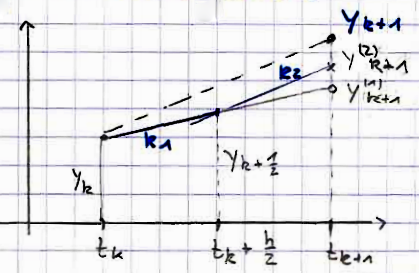
\includegraphics[scale=0.42]{5-EDO-eulercauch.png}
    \end{wrapfigure}

La méthode d'Euler-Cauchy est un \textbf{schéma d'ordre 2}.


\vspace{5cm}
COURS INCOMPLET.

